\chapter{Laboratorio 5}
Il primo circuito visto a lezione è come utilizzare il 555 per effettuare switch debouncing. Vediamone lo schema circuitale ed una sua immagine:
\begin{figure}[h!]
	\centering
	\begin{minipage}{.45\textwidth}
		\scalebox{.47}{
			\begin{circuitikz}
				%Main dip package
				\draw (0,0) node[dipchip,num pins=8, hide numbers, external pins width=0.1, scale=3, external pad fraction=6](C){LM555};
				%Pin names
				\node [right] at (C.bpin 1) {GND};
				\node [right] at (C.bpin 2) {Trigger};
				\node [right] at (C.bpin 3) {Output};
				\node [right] at (C.bpin 4) {Reset};
				\node [left] at (C.bpin 5) {Control Voltage};
				\node [left] at (C.bpin 6) {Threshold};
				\node [left] at (C.bpin 7) {Discharge};
				\node [left] at (C.bpin 8) {$V_{CC}$};
				%Connections
				\draw (C.pin 1) -- ++(-2.9,0) ++(-.1,0) node[jump crossing](crgnd){} ++(-.1,0) -- ++(-.9,0) -- ++(0,-6) node[ground]{};
				\draw (C.pin 8) -- ++(2,0) coordinate(vcc) -- ++(0,1.35) node[vcc]{$V_{CC}$};
				\draw (C.pin 7) -- ++(2,0) coordinate(dsc) to[R=$R$] (vcc);
				\draw (C.pin 6) -- ++(2,0) coordinate(trs) -- (dsc);
				\draw (trs) -- ++(2,0) to[C=$C$] ++(0,-2.68) node[ground]{};
				\draw (C.pin 5) -- ++(2,0) to[C=$C_2$] ++(0,-1) node[ground]{};
				\draw (C.pin 4) -- ++(-1.5,0) -- ++(0,3) to[crossing] ++(0,.72) to[crossing] ++ (0,2.64) node[vcc]{$V_{CC}$};
				\draw (C.pin 3) to[short, -o] ++(-1,0) ++(0,.1) node[above]{$v_{out}$};
				\draw (C.pin 2) -- ++(-3,0) coordinate(vin);
				\draw (vin) to[nopb=$B$] ++(0,-4.32) node[ground]{};
				\draw (vin) to[R=$R$] (crgnd) -- ++(0,1.33) node[vcc]{$V_{CC}$};
				\draw[thick] (-7.5,-5.3) rectangle (8,5.9);
			\end{circuitikz}
		}
	\end{minipage}\qquad
	\begin{minipage}{.45\textwidth}
		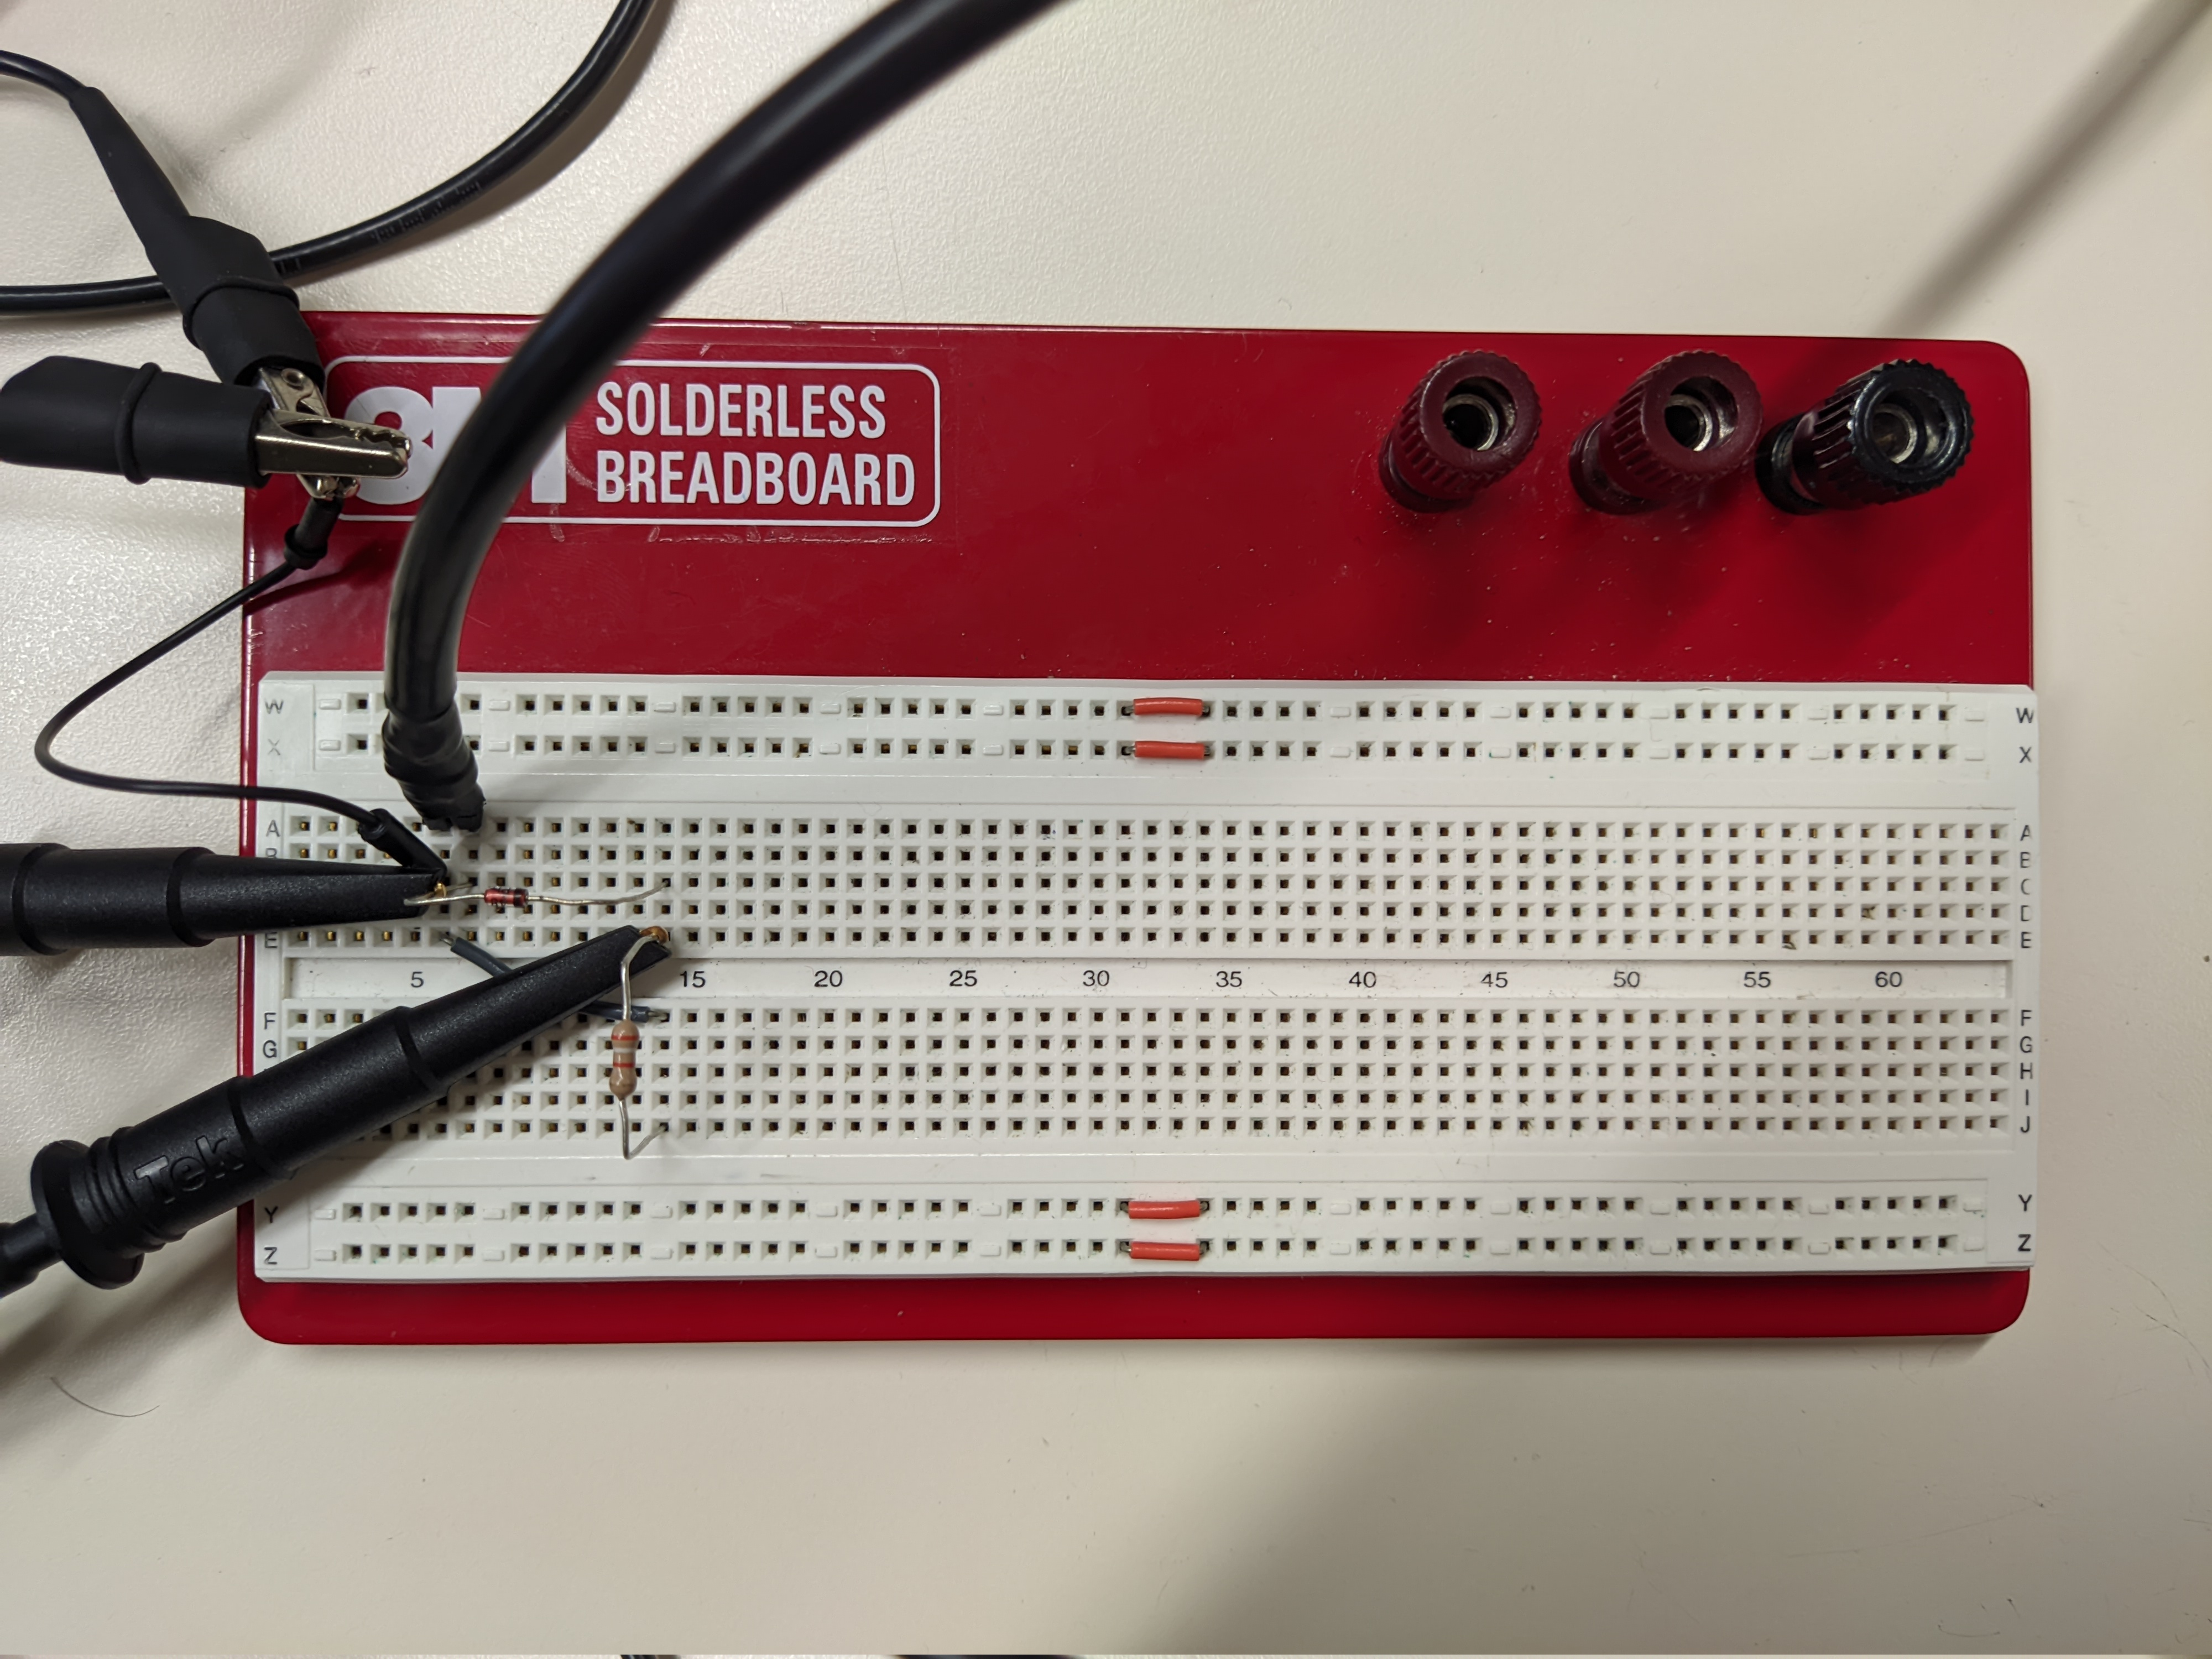
\includegraphics[width=\linewidth]{./ImageFiles/Laboratorio 5/CIR1.jpg}
	\end{minipage}
	\caption{Schema circuitale e foto del circuito realizzato.}
	\label{fig:circuito_2}
\end{figure}
Questo circuito è praticamente identico all'ultimo circuito visto nella lezione precedente, con l'unica differenza riguardo alla sorgente dell'impulso fornito in ingresso all'integrato \textbf{LM555}. Infatti precedentemente questa era fornita direttamente da un generatore di segnale dove ora invece è stato sostituito da un interruttore meccanico normalmente aperto. Questo è collegato ad un suo capo a massa, mentre sull'altro capo è collegato al pin di trigger ed a una resistenza. La resistenza è legata a $V_{CC}$ all'altro capo. La resistenza è quindi utilizzata come resistenza di pull-up, fornendo $V_{CC}$ al piedino del trigger quando l'interruttore è aperto e viene portata a massa dall'interruttore quando quest'ultimo viene chiuso, dove la R si comporta come limitatore di corrente\todo{Mi fa schifo come frase}.

Il problema dello switch bouncing\todo{altra bruttura} deriva dalla sua struttura meccanica interna. Infatti, quando questo viene chiuso o aperto, proprio per come è costruito internamente, questo tende ad oscillare per un certo periodo causando un "treno" di impulsi che vengono visti dall'elettronica davanti come un set continuo di pressioni e rilasci invece che una pressione singola come invece avviene nella realtà. Questo tipo di circuito quindi si comporta come da "filtro" per questo comportamento, fornendo in uscita solo il primo cambio di pendenza sul piedino del trigger invece di tutti gli eventi spuri generati all'ingresso, visto che la durata dell'evento di uscita è determinato puramente da R e da C e non dal numero di impulsi all'ingresso del 555.